\chapter{Biome und Dekorationen}
\label{ch:advmap/biomesdeco}

Biome\index{biom@Biom} und Dekorationen\index{dekoration@Dekoration}
registrieren zu können, ist entscheidend für eine interessante und
abwechslungsreiche Spielwelt. Dieses Kapitel zeigt, wie du Biome
registrierst, ihre Verteilung steuerst und Dekorationen in Biomen
platzierst.

\section{Was sind Biome?}\label{was-sind-biome}

Ein Biom ist in Luanti eine bestimmte Umgebung in der Spielwelt. Beim
Registrieren eines Bioms legst du fest, welche Nodes bei der
Kartengenerierung\index{kartengenerierung@Kartengenerierung} darin
vorkommen. Zu den Node-Arten, die sich am häufigsten von Biom zu Biom
unterscheiden, gehören:

\begin{itemize}
\tightlist
\item
  Oberflächen-Node (\emph{top node}): der Node, der an der Oberfläche am
  häufigsten vorkommt. Ein bekanntes Beispiel ist „Erde mit Gras`` aus
  Minetest Game.
\item
  Füll-Node (\emph{filler node}): die Schicht direkt unter dem
  Oberflächen-Node. In Biomen mit Gras ist das oft Erde.
\item
  Stein-Node: der Node, den man unter der Erde am häufigsten sieht.
\item
  Wasser-Node: meist eine Flüssigkeit; dieser Node erscheint dort, wo
  man Gewässer erwartet.
\end{itemize}

Auch andere Node-Arten können sich zwischen Biomen unterscheiden. So
lassen sich im selben Spiel sehr unterschiedliche Umgebungen schaffen.

\section{Platzierung von Biomen}\label{platzierung-von-biomen}

\subsection{Wärme und Feuchtigkeit}\label{wuxe4rme-und-feuchtigkeit}

Ein Biom nur zu registrieren, genügt nicht; du musst auch festlegen, wo
es im Spiel vorkommen kann. Dazu bekommt jedes Biom einen Wert für Wärme
(\emph{heat}) und Feuchtigkeit (\emph{humidity}).

Überlege dir diese Werte gut, denn sie bestimmen, welche Biome
aneinandergrenzen können. Bei schlechter Wahl grenzt eine heiße Wüste
womöglich an einen Gletscher, und es entstehen andere unwahrscheinliche
Kombinationen, die du lieber vermeiden möchtest.

Im Spiel liegen Wärme und Feuchtigkeit an jedem Punkt der Karte meist
zwischen 0 und 100. Die Werte ändern sich allmählich, während man sich
über die Karte bewegt. An jedem Punkt entsteht das registrierte Biom,
dessen Wärme- und Feuchtigkeitswerte denen an dieser Stelle der Karte am
nächsten kommen.

Da sich Wärme und Feuchtigkeit nur allmählich ändern, solltest du die
Werte eines Bioms an dem ausrichten, was man von seiner Umgebung
erwarten würde. Zum Beispiel:

\begin{itemize}
\tightlist
\item
  Eine Wüste hat hohe Wärme und niedrige Feuchtigkeit.
\item
  Ein verschneiter Wald hat niedrige Wärme und mittlere Feuchtigkeit.
\item
  Ein Sumpf hat meist hohe Feuchtigkeit.
\end{itemize}

Solange du eine vielfältige Auswahl an Biomen hast, ergibt sich so in
der Praxis meist ein logischer Übergang zwischen benachbarten Biomen.

\subsection{Grenzen mit Voronoi-Diagrammen
veranschaulichen}\label{grenzen-mit-voronoi-diagrammen-veranschaulichen}

\begin{figure}
\centering
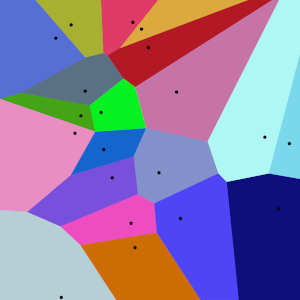
\includegraphics[width=5cm,height=\textheight,keepaspectratio,alt={Voronoi-Diagramm: Jede Fläche enthält die Punkte, die ihrem Mittelpunkt am nächsten liegen. Bild: Balu Ertl, CC BY-SA 4.0}]{bilder/biomes_voronoi.png}
\caption{Voronoi-Diagramm: Jede Fläche enthält die Punkte, die ihrem
Mittelpunkt am nächsten liegen. Bild: Balu Ertl, CC BY-SA 4.0}
\end{figure}

Wärme- und Feuchtigkeitswerte lassen sich leichter feinabstimmen, wenn
du die Beziehungen zwischen deinen Biomen sichtbar machst. Das ist
besonders wichtig, wenn du einen kompletten eigenen Satz an Biomen
erstellst, kann aber auch beim Ergänzen eines bestehenden Satzes helfen.

Am einfachsten machst du sichtbar, welche Biome aneinandergrenzen
können, mit einem
Voronoi-Diagramm.\index{voronoi-diagramm@Voronoi-Diagramm} Es zeigt für
jede Stelle eines zweidimensionalen Diagramms, welchem Punkt sie am
nächsten liegt.

Ein Voronoi-Diagramm zeigt, wo Biome, die aneinandergrenzen sollten, es
nicht tun -- und wo Biome aneinandergrenzen, die es nicht sollten.
Außerdem gibt es einen groben Eindruck davon, wie häufig Biome im Spiel
sein werden: Große und zentral liegende Biome sind häufiger als kleine
oder solche am Rand des Diagramms.

Dazu setzt du für jedes Biom einen Punkt anhand seiner Wärme und
Feuchtigkeit, mit der Wärme auf der x-Achse und der Feuchtigkeit auf der
y-Achse. Dann teilst du das Diagramm in Flächen ein, sodass jede Stelle
einer Fläche näher an deren Punkt liegt als an jedem anderen Punkt des
Diagramms.

Jede Fläche steht für ein Biom. Haben zwei Flächen eine gemeinsame
Grenze, können die zugehörigen Biome im Spiel nebeneinander liegen. Wie
lang die gemeinsame Grenze im Vergleich zu den Grenzen mit anderen
Flächen ist, verrät, wie häufig die beiden Biome voraussichtlich
nebeneinander vorkommen.

\subsection{Voronoi-Diagramme mit GeoGebra
erstellen}\label{voronoi-diagramme-mit-geogebra-erstellen}

Voronoi-Diagramme kannst du von Hand zeichnen oder mit Programmen wie
GeoGebra\footnote{\url{https://www.geogebra.org}} erstellen.

\begin{enumerate}
\def\labelenumi{\arabic{enumi}.}
\item
  Lege Punkte an, indem du in der Werkzeugleiste das Punktwerkzeug
  wählst (Symbol: ein Punkt mit „A``) und in das Diagramm klickst. Du
  kannst Punkte verschieben oder ihre Position in der linken
  Seitenleiste genau eingeben. Gib jedem Punkt außerdem eine
  Beschriftung, das macht es übersichtlicher.
\item
  Erzeuge dann das Voronoi-Diagramm, indem du in das Eingabefeld der
  linken Seitenleiste diese Funktion eingibst:

\begin{Shaded}
\begin{Highlighting}[]
\NormalTok{Voronoi(\{ A, B, C, D, E \})}
\end{Highlighting}
\end{Shaded}

  In den geschweiften Klammern stehen alle Punkte, durch Kommas
  getrennt.
\item
  Fertig! Du hast jetzt ein Voronoi-Diagramm, dessen Punkte du
  verschieben kannst.
\end{enumerate}

\section{Ein Biom registrieren}\label{ein-biom-registrieren}

Der folgende Code registriert ein einfaches Biom namens
\texttt{grasslands}:

\begin{Shaded}
\begin{Highlighting}[]
\VariableTok{core}\OperatorTok{.}\NormalTok{register\_biome}\OperatorTok{(\{}
    \VariableTok{name} \OperatorTok{=} \StringTok{"grasslands"}\OperatorTok{,}
    \VariableTok{node\_top} \OperatorTok{=} \StringTok{"default:dirt\_with\_grass"}\OperatorTok{,}
    \VariableTok{depth\_top} \OperatorTok{=} \DecValTok{1}\OperatorTok{,}
    \VariableTok{node\_filler} \OperatorTok{=} \StringTok{"default:dirt"}\OperatorTok{,}
    \VariableTok{depth\_filler} \OperatorTok{=} \DecValTok{3}\OperatorTok{,}
    \VariableTok{y\_max} \OperatorTok{=} \DecValTok{1000}\OperatorTok{,}
    \VariableTok{y\_min} \OperatorTok{=} \OperatorTok{{-}}\DecValTok{3}\OperatorTok{,}
    \VariableTok{heat\_point} \OperatorTok{=} \DecValTok{50}\OperatorTok{,}
    \VariableTok{humidity\_point} \OperatorTok{=} \DecValTok{50}\OperatorTok{,}
\OperatorTok{\})}
\end{Highlighting}
\end{Shaded}

Dieses Biom hat an der Oberfläche eine Schicht „Erde mit Gras`` und
darunter drei Schichten Erde. Es gibt keinen Stein-Node an; unter der
Erde liegt daher der Node, der als Mapgen-Alias
\texttt{mapgen\_\allowbreak{}stone} registriert ist.

Beim Registrieren eines Bioms gibt es viele Optionen; sie sind wie immer
in der Lua-API-Referenz\footnote{\url{https://api.luanti.org/definition-tables/\#biome-definition}}
dokumentiert.

Du musst nicht für jedes Biom jede Option angeben. Fehlt aber eine
bestimmte Option oder ein passender Mapgen-Alias, kann es zu Fehlern bei
der Kartengenerierung kommen.

\section{Was sind Dekorationen?}\label{was-sind-dekorationen}

Dekorationen sind Nodes oder Schematics, die bei der Kartengenerierung
auf der Karte platziert werden. Typische Beispiele sind Blumen, Büsche
und Bäume. Kreativere Einsätze sind etwa Eiszapfen oder Stalagmiten in
Höhlen, unterirdische Kristallformationen oder sogar kleine Gebäude.

Dekorationen lassen sich auf bestimmte Biome, Höhen oder
Untergrund-Nodes beschränken. Oft gestalten sie die Umgebung eines
Bioms, indem sie für bestimmte Pflanzen, Bäume oder andere Merkmale
sorgen.

\section{Eine einfache Dekoration
registrieren}\label{eine-einfache-dekoration-registrieren}

Einfache Dekorationen platzieren bei der Kartengenerierung einzelne
Nodes. Du gibst an, welcher Node als Dekoration platziert wird, wo er
platziert werden darf und wie häufig er vorkommt.

Zum Beispiel:

\begin{Shaded}
\begin{Highlighting}[]
\VariableTok{core}\OperatorTok{.}\NormalTok{register\_decoration}\OperatorTok{(\{}
    \VariableTok{deco\_type} \OperatorTok{=} \StringTok{"simple"}\OperatorTok{,}
    \VariableTok{place\_on} \OperatorTok{=} \OperatorTok{\{} \StringTok{"base:dirt\_with\_grass"} \OperatorTok{\},}
    \VariableTok{sidelen} \OperatorTok{=} \DecValTok{16}\OperatorTok{,}
    \VariableTok{fill\_ratio} \OperatorTok{=} \DecValTok{0.1}\OperatorTok{,}
    \VariableTok{biomes} \OperatorTok{=} \OperatorTok{\{} \StringTok{"grassy\_plains"} \OperatorTok{\},}
    \VariableTok{y\_max} \OperatorTok{=} \DecValTok{200}\OperatorTok{,}
    \VariableTok{y\_min} \OperatorTok{=} \DecValTok{1}\OperatorTok{,}
    \VariableTok{decoration} \OperatorTok{=} \StringTok{"plants:grass"}\OperatorTok{,}
\OperatorTok{\})}
\end{Highlighting}
\end{Shaded}

Hier wird der Node \texttt{plants:grass} im Biom
\texttt{grassy\_\allowbreak{}plains} auf
\texttt{base:dirt\_\allowbreak{}with\_\allowbreak{}grass} platziert,
zwischen den Höhen \texttt{y = 1} und \texttt{y = 200}.

\texttt{fill\_\allowbreak{}ratio} bestimmt, wie häufig die Dekoration
vorkommt; höhere Werte bis 1 führen zu sehr vielen Dekorationen.
Alternativ kannst du die Platzierung über Rauschparameter (\emph{noise
parameters}) steuern.

\section{Eine Schematic-Dekoration
registrieren}\label{eine-schematic-dekoration-registrieren}

Schematic-Dekorationen funktionieren ganz ähnlich wie einfache
Dekorationen, platzieren aber eine Schematic statt eines einzelnen
Nodes. Zum Beispiel:

\begin{Shaded}
\begin{Highlighting}[]
\VariableTok{core}\OperatorTok{.}\NormalTok{register\_decoration}\OperatorTok{(\{}
    \VariableTok{deco\_type} \OperatorTok{=} \StringTok{"schematic"}\OperatorTok{,}
    \VariableTok{place\_on} \OperatorTok{=} \OperatorTok{\{} \StringTok{"base:desert\_sand"} \OperatorTok{\},}
    \VariableTok{sidelen} \OperatorTok{=} \DecValTok{16}\OperatorTok{,}
    \VariableTok{fill\_ratio} \OperatorTok{=} \DecValTok{0.0001}\OperatorTok{,}
    \VariableTok{biomes} \OperatorTok{=} \OperatorTok{\{} \StringTok{"desert"} \OperatorTok{\},}
    \VariableTok{y\_max} \OperatorTok{=} \DecValTok{200}\OperatorTok{,}
    \VariableTok{y\_min} \OperatorTok{=} \DecValTok{1}\OperatorTok{,}
    \VariableTok{schematic} \OperatorTok{=} \VariableTok{core}\OperatorTok{.}\NormalTok{get\_modpath}\OperatorTok{(}\StringTok{"plants"}\OperatorTok{)}
        \OperatorTok{..} \StringTok{"/schematics/cactus.mts"}\OperatorTok{,}
    \VariableTok{flags} \OperatorTok{=} \StringTok{"place\_center\_x, place\_center\_z"}\OperatorTok{,}
    \VariableTok{rotation} \OperatorTok{=} \StringTok{"random"}\OperatorTok{,}
\OperatorTok{\})}
\end{Highlighting}
\end{Shaded}

Hier wird die Schematic \texttt{cactus.\allowbreak{}mts} in Wüstenbiomen
platziert. Du musst den Pfad zu einer Schematic angeben; in diesem Fall
liegt sie in einem eigenen Schematic-Verzeichnis innerhalb des Mods.

Das Beispiel setzt außerdem Flags, um die Schematic mittig zu
platzieren, und eine zufällige Drehung. Zufällig gedrehte Schematics
sorgen für mehr Abwechslung, wenn sie nicht symmetrisch sind.

\section{Mapgen-Aliase}\label{mapgen-aliase}

Bestehende Spiele bringen bereits passende Mapgen-Aliase mit. Eigene
musst du nur registrieren, wenn du ein eigenes Spiel entwickelst.

Mapgen-Aliase geben dem Kartengenerator der Engine Informationen und
werden so registriert:

\begin{Shaded}
\begin{Highlighting}[]
\VariableTok{core}\OperatorTok{.}\NormalTok{register\_alias}\OperatorTok{(}\StringTok{"mapgen\_stone"}\OperatorTok{,} \StringTok{"base:smoke\_stone"}\OperatorTok{)}
\end{Highlighting}
\end{Shaded}

Mindestens diese solltest du registrieren:

\begin{itemize}
\tightlist
\item
  \texttt{mapgen\_\allowbreak{}stone}
\item
  \texttt{mapgen\_\allowbreak{}water\_\allowbreak{}source}
\item
  \texttt{mapgen\_\allowbreak{}river\_\allowbreak{}water\_\allowbreak{}source}
\end{itemize}

Legst du nicht für alle Biome Höhlenflüssigkeiten fest, solltest du
außerdem registrieren:

\begin{itemize}
\tightlist
\item
  \texttt{mapgen\_\allowbreak{}lava\_\allowbreak{}source}
\end{itemize}
